% =============================================================================
% Kapitel 2: Systemarchitektur von ROSI
% =============================================================================

\section{Systemarchitektur von ROSI}
\label{sec:architektur}

Die untersuchten Fehlerklassen lassen sich erst mit Kenntnis der konkreten Prozess- und
Speicherarchitektur einordnen. Dieser Abschnitt beschreibt die für die Failure Cases
relevanten Bausteine: die Prozess-Topologie, die Verarbeitungspipeline mit ihrem
Worker-Pool und das Shared-Memory-basierte Speichermanagement.

\subsection{Prozess-Topologie}
\label{sec:architektur-topologie}

ROSI ist bewusst als Multiprocessing-System ausgelegt, um den \textit{Global Interpreter
Lock} von Python zu umgehen und große Bilddatenmengen nicht durch teure
Inter-Prozess-Kommunikation zu blockieren. Der Startprozess \texttt{main.py} teilt das
System in vier langlebige Service-Prozesse auf, die über threadsichere Queues und
Event-Primitive kommunizieren (Abbildung~\ref{fig:topologie}). Der
\texttt{InspectionDataHandler} erzeugt fortlaufend leere Daten-Container und schiebt sie
über eine begrenzte Queue in das System; ist die Queue voll, blockiert er und wirkt so als
systemweites Backpressure-Ventil gegen unbegrenzte Speicherallokation. Der
\texttt{FrameGrabber} bindet die Kamerahardware an, schreibt die rohen Pixeldaten in
Shared-Memory-Blöcke und reicht Referenzen darauf an den \texttt{PipelineManager} weiter.
Dieser orchestriert die eigentliche Verarbeitung. Der \texttt{LoggerProcess} nimmt die
Lognachrichten aller Prozesse über eine zentrale Queue entgegen und schreibt sie
asynchron nach PostgreSQL, sodass I/O-Latenzen die Bildverarbeitung nicht ausbremsen.

Für die Fehlertoleranz ist eine Eigenschaft dieser Topologie zentral:
\texttt{main.py} überwacht zur Laufzeit ausschließlich den \texttt{PipelineManager}
über einen Poll im Sekundentakt. Die drei übrigen Service-Prozesse laufen nach
erfolgreichem Start ohne jede Laufzeit-Supervision. Genau an dieser Lücke setzt
Case~1 (Abschnitt~\ref{sec:case1}) an; in Abbildung~\ref{fig:topologie} sind die
unüberwachten Prozesse rot markiert.

\begin{figure}[htbp]
    \centering
    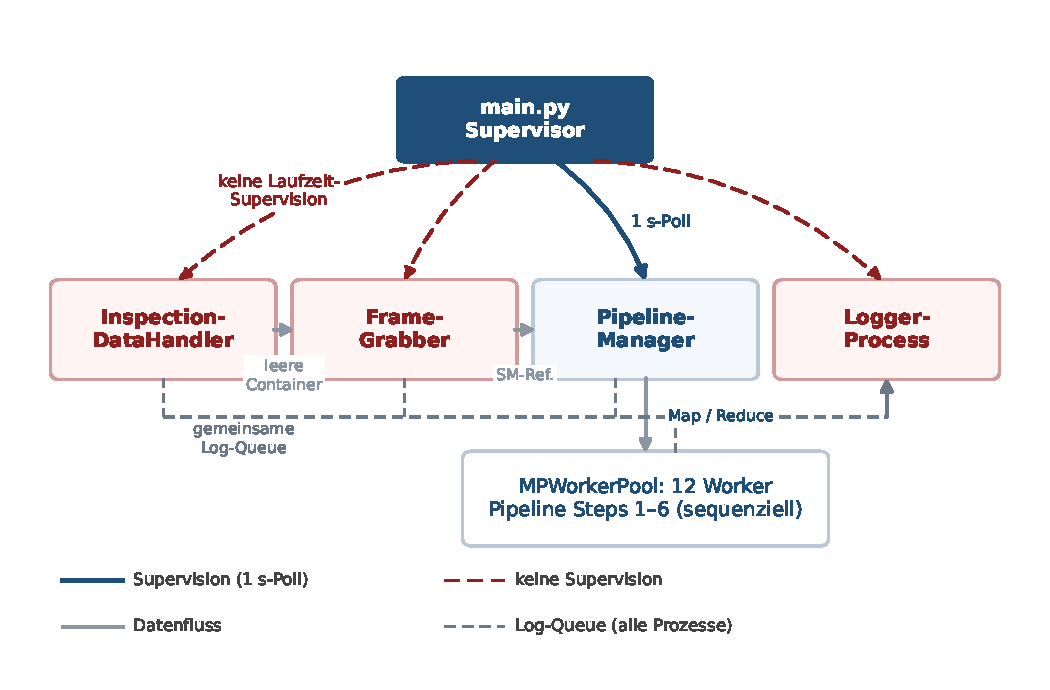
\includegraphics[width=0.95\textwidth]{assets/img/topology.pdf}
    \caption[Prozess-Topologie von ROSI]{Prozess-Topologie von ROSI.
        \texttt{main.py} überwacht zur Laufzeit nur den \texttt{PipelineManager}
        (1\,s-Poll); die drei rot markierten Service-Prozesse laufen ohne
        Laufzeit-Supervision (Case~1). Graue Pfeile zeigen den Datenfluss; große
        Bilddaten wandern nicht durch die Queues, sondern als
        Shared-Memory-Referenzen. Alle Prozesse loggen über die gemeinsame Log-Queue.}
    \source{Eigene Darstellung}
    \label{fig:topologie}
\end{figure}

\subsection{Verarbeitungspipeline und Worker-Pool}
\label{sec:architektur-pipeline}

Der \texttt{PipelineManager} führt jede Inspektion durch eine streng sequenzielle
Pipeline aus sechs Schritten. Rechenintensive Schritte -- KI-Inferenz, Geometrievermessung
und Bildkompression -- lagert er über ein Map-Reduce-Muster in den \texttt{MPWorkerPool}
mit zwölf Worker-Prozessen aus: Ein Schritt wird in Teiljobs zerlegt (Map), auf freie
Worker verteilt und das Ergebnis wieder zusammengeführt (Reduce). Ein Scheduler wählt
dabei den Worker mit der kürzesten Job-Queue. Zwei Hintergrund-Threads ergänzen den Pool:
Der \texttt{ResultCollector} sammelt die Teilergebnisse nicht blockierend ein und
benachrichtigt die Pipeline erst, wenn alle Teiljobs abgeschlossen sind; ein
\texttt{HealthMonitor} überwacht die Heartbeats der Worker und startet einen nicht mehr
antwortenden Worker neu. Diese Worker-Überwachung ist damit deutlich engmaschiger als die
Supervision der Service-Prozesse -- ein Gefälle, das für die Fehlerbilder in
Kapitel~\ref{sec:cases} bedeutsam ist.

Tabelle~\ref{tab:pipeline} fasst die sechs Schritte mit ihren im Referenzlauf gemessenen
Laufzeiten zusammen. Die kurzen, planbaren Schrittdauern sind später die Grundlage der
Timing-Analyse in Case~5 (Abschnitt~\ref{sec:case5}).

\begin{table}[htbp]
    \centering
    \caption{Schritte der Verarbeitungspipeline mit Referenz-Laufzeiten}
    \label{tab:pipeline}
    \begin{tabularx}{\textwidth}{cl>{\raggedright\arraybackslash}X>{\raggedleft\arraybackslash}p{20mm}}
        \hline
        \textbf{Step} & \textbf{Ausführung} & \textbf{Aufgabe} & \textbf{$\varnothing$ Dauer} \\
        \hline
        1 & lokal    & Warten auf neue Inspektionsdaten (\texttt{wait\_for\_new\_inspection}) & 10--20\,ms \\
        2 & lokal    & Geometrievermessung                     & 25--70\,ms \\
        3 & lokal    & Zuschnitt der Region of Interest         & 5--15\,ms \\
        4 & parallel & Defekterkennung (klassisch + KI) und Bildkodierung & 170--220\,ms \\
        5 & parallel & Merkmalsextraktion und Bildspeicherung   & 50--110\,ms \\
        6 & lokal    & Persistierung nach PostgreSQL (Django-ORM) & 5--110\,ms \\
        \hline
    \end{tabularx}
\end{table}

\subsection{Speichermanagement: Shared Memory und Zero-Copy}
\label{sec:architektur-speicher}

Das kritischste Entwurfsmuster von ROSI ist die Vermeidung teurer Serialisierung großer
Bild-Arrays. Bilddaten wandern nie durch Queues, sondern werden über
\texttt{multiprocessing.\allowbreak{}shared\_memory} in vom Betriebssystem verwaltete
RAM-Blöcke geschrieben; die Queues transportieren nur kleine Proxy-Objekte mit
Block-Referenz, Form und Datentyp. Ein Worker verbindet sich beim Zugriff mit dem Block und
liest die Daten ohne Kopie (Zero-Copy). Weil das Betriebssystem den Speicher verwaltet,
gilt ein striktes Ownership-Konzept: \texttt{close()} löst nur die lokale Bindung,
\texttt{destroy()} gibt den Block global frei und darf genau einmal am Ende einer
Inspektion aufgerufen werden. Ein zusätzlicher Worker-seitiger Garbage Collector zerstört
Blöcke, auf die seit mehr als zehn Sekunden kein Zugriff erfolgte, um ein Volllaufen des
flüchtigen Speichers zu verhindern.

Bild-Archiv und Shared-Memory-Blöcke liegen auf getrennten Pfaden, teilen sich physisch
aber denselben Arbeitsspeicher: Das Bild-Archiv liegt in Produktion auf einer
tmpfs-RAM-Disk, die Shared-Memory-Blöcke unter \texttt{/dev/shm}. Diese gemeinsame
Ressource ist Ausgangspunkt von Case~2 (Abschnitt~\ref{sec:case2}), das
zehnsekündige Freigabeintervall Gegenstand der Hypothese in Case~5
(Abschnitt~\ref{sec:case5}).
